% id: 34-04
% book: 100발100중 3-2 기말 · 01 3-2 기말(원의 성질·통계·부록)
% section: 실전 문제 1회
% figure: crop:fig-34-04.png
% answer: ⑤
% answer_source: 답지(빠른정답)
% variant_level: 0 (원본 전사)
% 이 파일은 build.mjs 가 items.json 에서 만든다. 고칠 때는 items.json 을 고친다.
\smash{\raisebox{1.5mm}{\dmkichul{100발100중 3-2 기말 34쪽 04번}}}
\noindent\begin{minipage}[t]{0.58\linewidth}\vspace{0pt}\raggedright 그림과 같이 오각형~$\pt{ABCDE}$가 원~$\pt{O}$에 내접하고 $\angle\pt{BAE}=100^\circ$, $\angle\pt{CDE}=110^\circ$일 때, $\angle x$의 크기는?\end{minipage}\hfill\begin{minipage}[t]{0.4\linewidth}\vspace{0pt}\centering 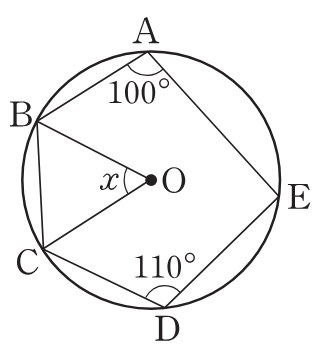
\includegraphics[width=76.5pt]{figures/fig-34-04.png}\end{minipage}\par
\begin{choicesii}{$30^\circ$}{$40^\circ$}{$45^\circ$}{$50^\circ$}{$60^\circ$}\end{choicesii}
